\documentclass[12pt]{article}
\usepackage[utf8]{inputenc}
\usepackage{geometry}
\usepackage{multicol}
\usepackage{listings}
\usepackage{color}
\usepackage{graphicx}
\usepackage{mathrsfs}
\usepackage{hyperref}

\usepackage{lipsum}
\usepackage{transparent}
\usepackage{eso-pic}

\usepackage{svg}
\usepackage{amsmath,amssymb,amsthm,enumitem}
\usepackage[makeroom]{cancel}
\geometry{margin=2cm}
%\geometry{left=2cm, top=4cm}

\usepackage{xcolor}

\usepackage{styles/style}

\newcommand\rurl[1]{%
	\href{http://#1}{\nolinkurl{#1}}%
}

%size 8.5 x 11 in
\title{Pruebas}
\author{rafael.rvp98 }
\date{September 2018}

\begin{document}
%\maketitle

\newgeometry{margin = 0in}
%Barra Azul
\hspace*{-0.9cm}
\vspace{-3mm}
\colorbox{azul2}{
	\makebox[8.5in][l]{
		\shortstack[l]{
			%\vspace{1.75in}\\
			%\vspace{0.1in}\\
			%
\includegraphics[scale=0.05]{images/cerebro-transparente}\\
			\vspace{2.75in}
			%\vspace{1.75in}
			%\vspace{0.1in}
		}
	}
}

%Barra Blanca
\hspace*{-0.9cm}
\colorbox{blanco}{\makebox[8.5in][r]{\vspace{1mm}}}\\

\hspace*{-0.9cm}
\colorbox{white}{\makebox[8.25in][l]{\hfill\shortstack[r]{\fontsize{36}{36}\rmfamily\color{azul1}Introducción a Statistical\vspace{0.3cm}\\ \fontsize{36}{36}\rmfamily\color{azul1}Machine Learning}}}

\hspace*{-0.9cm}
\colorbox{blanco}{\makebox[8.5in][r]{\vspace{0.02mm}}}\\

%Barra Azul

%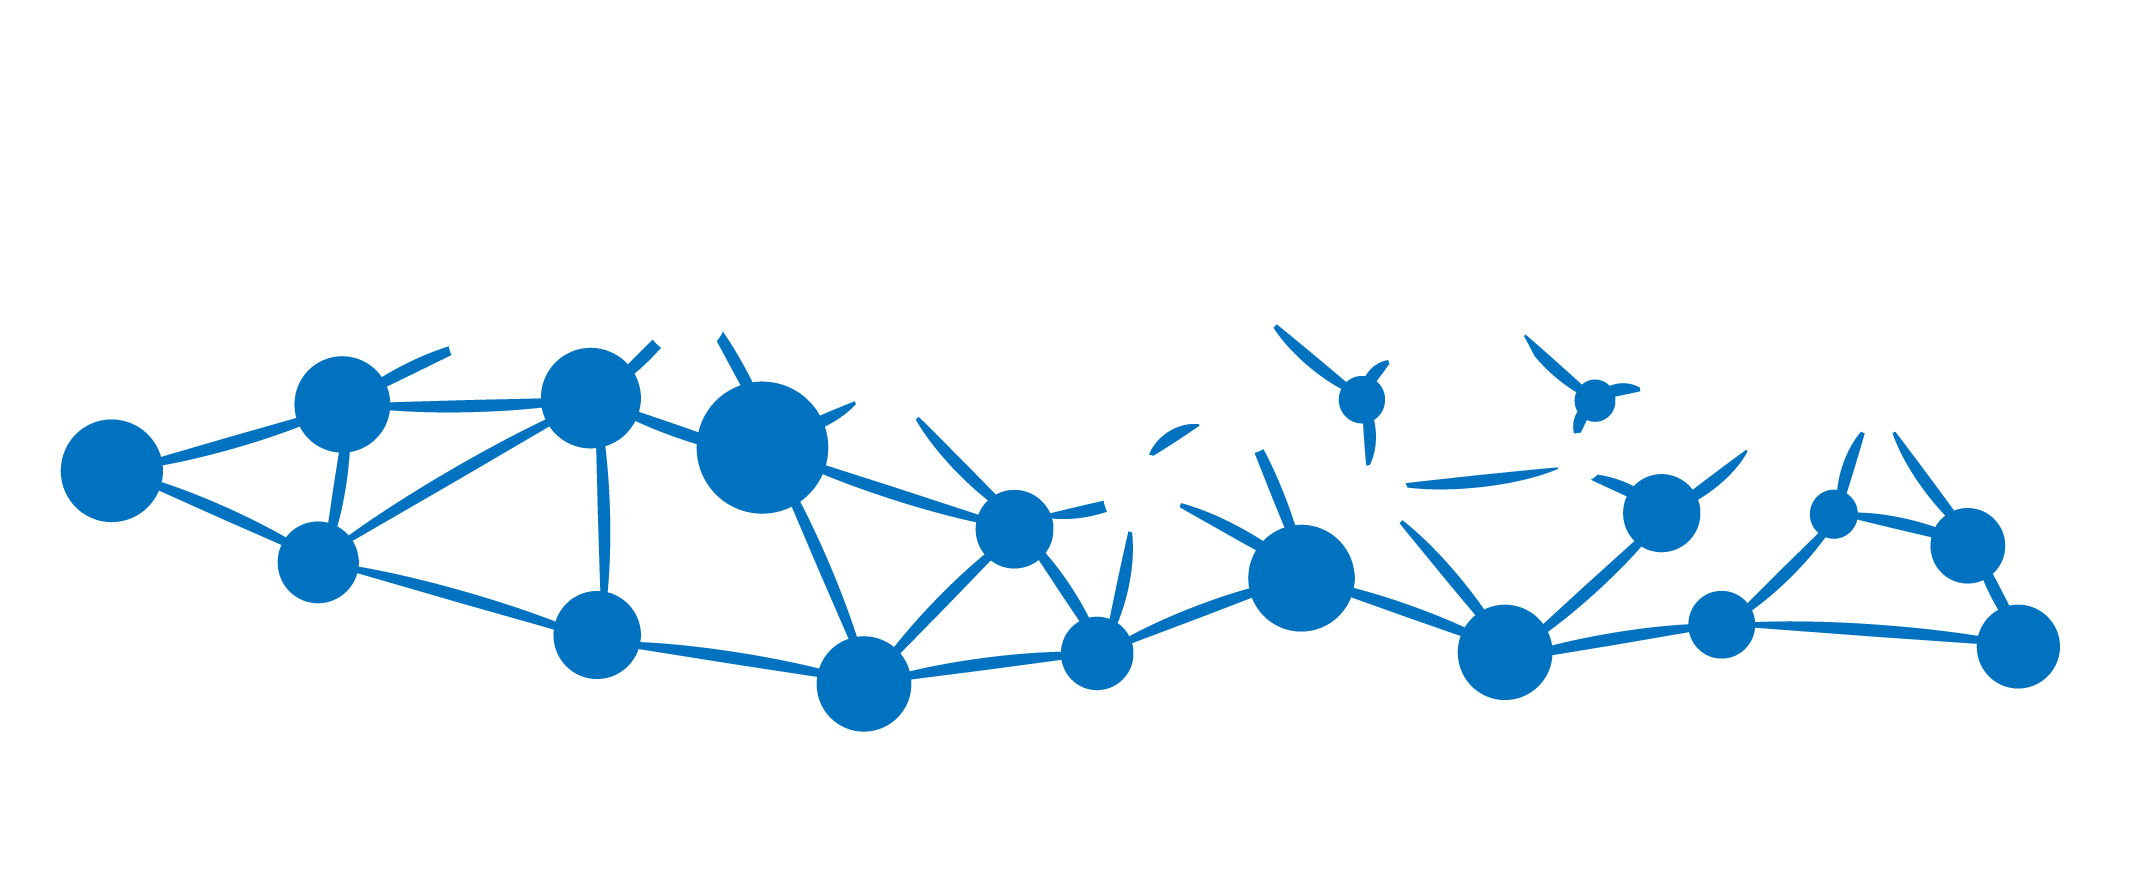
\includegraphics[width=3.09in]{images/transparente-tiny.png}
\vspace{-4.5mm}
\hspace*{-0.76cm}
%\colorbox{azul2}{\makebox[8.5in][r]{\shortstack[r]{\vspace{5.7in}}}}
\colorbox{azul2}{
	\makebox[8.35in][c]{
		\shortstack[c]{
			\vspace{0.31in}\\
			%\hspace{-1.8cm}
			\hspace{-0.8cm}
			\transparent{0.09}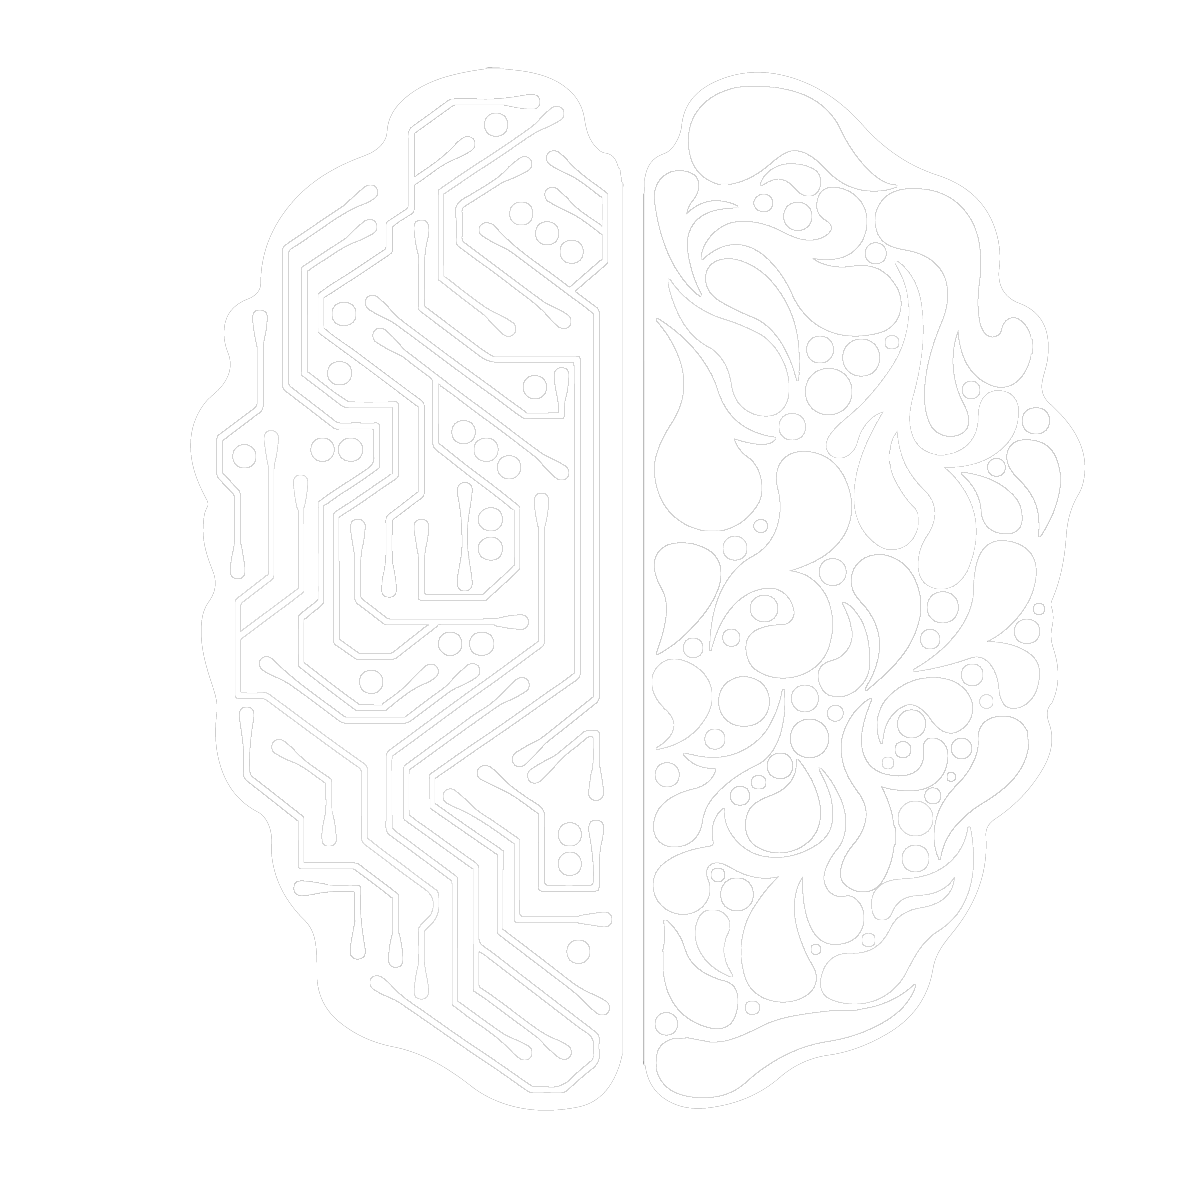
\includegraphics[scale=0.3]{images/cerebro-transparente-blanco}\\
			%\vspace{5.505in}
			\vspace{0.11in}
		}
	}
}

\vspace{-0.52mm}
%logos
\hspace{-0.9cm}
\colorbox{azul2}{\makebox[8.5in][c]{\shortstack[c]{
\includegraphics[scale=0.51]{images/pie-transparente.png}}}}

\newpage

\hspace*{1cm}
\colorbox{white}{%
	\shortstack[r]{
		\makebox[5.4in][r]{\shortstack[r]{\vspace{1in}}}\\
		\parbox{5.4in}{%
			\section*{\fontsize{25}{25}\rmfamily\color{celeste}1. Plan de Avance}
			\vspace*{1.5cm}
			\fontsize{15}{15}\rmfamily\color{celeste}
			\begin{enumerate}
				\item \textbf{Aprendizaje Supervisado}
				\begin{itemize}%
					\item Python para Machine Learning y Ciencia de Datos
					\item Métodos no Paramétricos
					\begin{itemize}%
						\item K Vecinos más Cercanos
						\item Árboles de Decisión y Random Forest
					\end{itemize}%
					\item Regresión Lineal y Métodos de Regularización
					\item Regresión Logística y Funciones de Activación
					\item \textbf{Proyecto de Medio Avance}
				\end{itemize}%
				\item \textbf{Redes Neuronales y Aprendizaje no Supervisado}
				\begin{itemize}%
					\item La Red Neuronal
					\item Reducción de Dimensionalidad
					\begin{itemize}%
						\item PCA
						\item TSNE
					\end{itemize}%
					\item Clustering
					\begin{itemize}%
						\item K-Prototype
						\item DBSCAN
					\end{itemize}%
					\item \textbf{Proyecto Final}
				\end{itemize}%
			\end{enumerate}%
		}%
		\\
		\makebox[5.2in][r]{\shortstack[r]{\vspace{3in}}}
	}
}
\hspace*{-2mm}
\hfill \colorbox{gris1}{%
	\shortstack[l]{
		\makebox[5.4in][l]{\shortstack[r]{\vspace{3.4 in}}}\\
		\fontsize{14}{14}\rmfamily\color{white}
		\parbox{5.4in}{%
			\begin{itemize}
				\setlength\itemsep{0.8mm}
				\item[] \textbf{11/sep - 13/sep}
				\item[] \textbf{18/sep - 21/sep}
				\\
				\\
				\vspace{0.2cm}
				\item[] \textbf{25/sep - 27/sep}
				\item[] \textbf{02/oct - 04/oct}
				\item[] \textbf{09/oct - 11/oct}
				\\
				\vspace{0.4cm}
				\item[] \textbf{16/oct - 18/oct}
				\item[] \textbf{23/oct - 25/oct}
				\\
				\\
				\vspace{0.3cm}
				\item[] \textbf{30/oct - 01/nov}
				\\
				\\
				\vspace{0.3cm}
				\item[] \textbf{06/nov - 08/nov}
			\end{itemize}
		}%
		\\
		vacio
		\makebox[5.2in][l]{\shortstack[r]{\vspace{3in}}}
	}
}%

\newpage

\hspace{-0.9cm}
\colorbox{gris1}{\makebox[2.2in][r]{\shortstack[r]{\vspace{11.61in}}}}
\hfill
%\hspace*{1cm}
\colorbox{white}{%
	\shortstack[r]{
		\makebox[5.4in][r]{\shortstack[r]{\vspace{1.98in}}}\\
		\parbox{5.4in}{%
			\section*{\fontsize{25}{25}\rmfamily\color{celeste}2. Requisitos}
			\vspace*{1.5cm}
			\fontsize{15}{15}\rmfamily\color{celeste}
			\begin{enumerate}%
				\item \textbf{Conocimiento}
				\begin{itemize}%
					\item Derivadas de Varias Variables
					\item Multiplicación Matricial
					\item Programación básica
					\begin{itemize}%
						\item Estructuras Condicionales
						\item Estructuras Repetitivas
						\item Lógica para Resolver Problemas Sencillos
					\end{itemize}%
				\end{itemize}%
				\item \textbf{Hardware}
				\begin{itemize}%
					\item De Preferencia Laptop con Python Instalado \\(Recomendación: Usar Anaconda)
					\item Procesador intel core i3 es suficiente.
				\end{itemize}%
			\end{enumerate}%
		}%
		\\
		\makebox[5.2in][r]{\shortstack[r]{\vspace{4.5in}}}
	}
} 

\newpage
\thispagestyle{empty}
\restoregeometry
\section*{\fontsize{25}{25}\rmfamily\color{celeste}3. Instructores}
\vspace*{1cm}
\fontsize{17}{17}\rmfamily\color{celeste}

\colorbox{white}{
	\makebox[7.5in][l]{
		\shortstack[c]{
			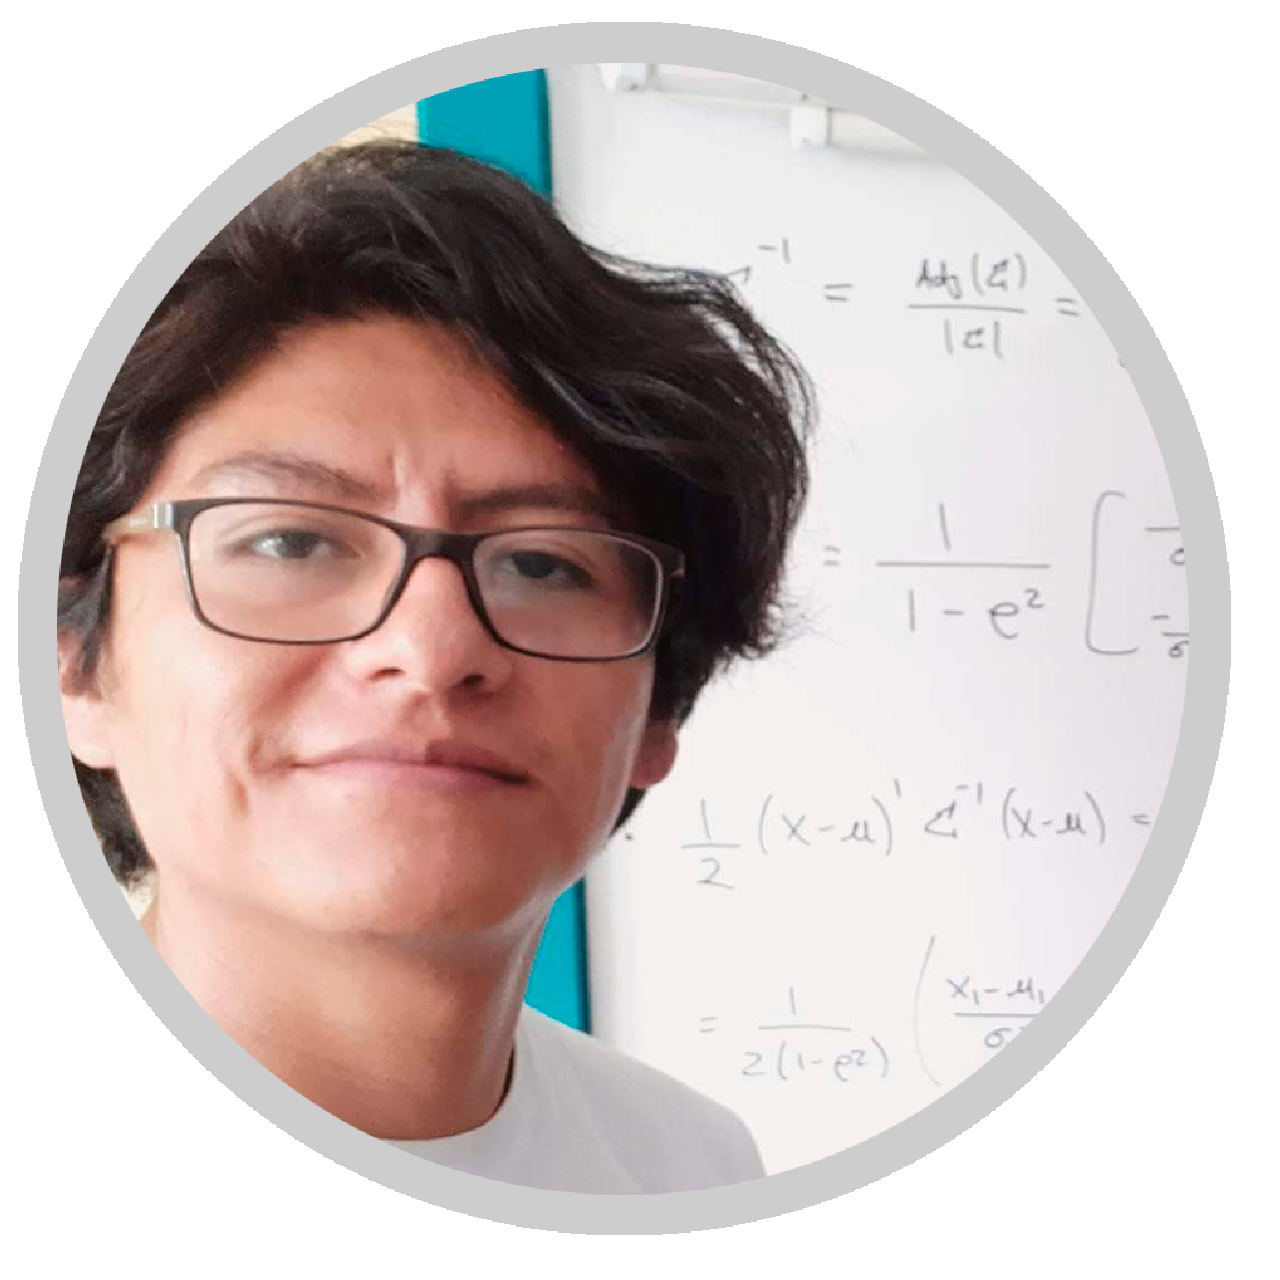
\includegraphics[scale=0.12]{images/Ayar-3}\\
			\textbf{Ayar Yuman Paco Sanizo}\\\\
			\href{https://www.linkedin.com/in/ayarpaco/}{
\includegraphics[scale=0.04]{images/linkedin_logo}} ayarpaco
		}
	}
}
\colorbox{white}{
	\makebox[7.5in][r]{
		\shortstack[c]{
			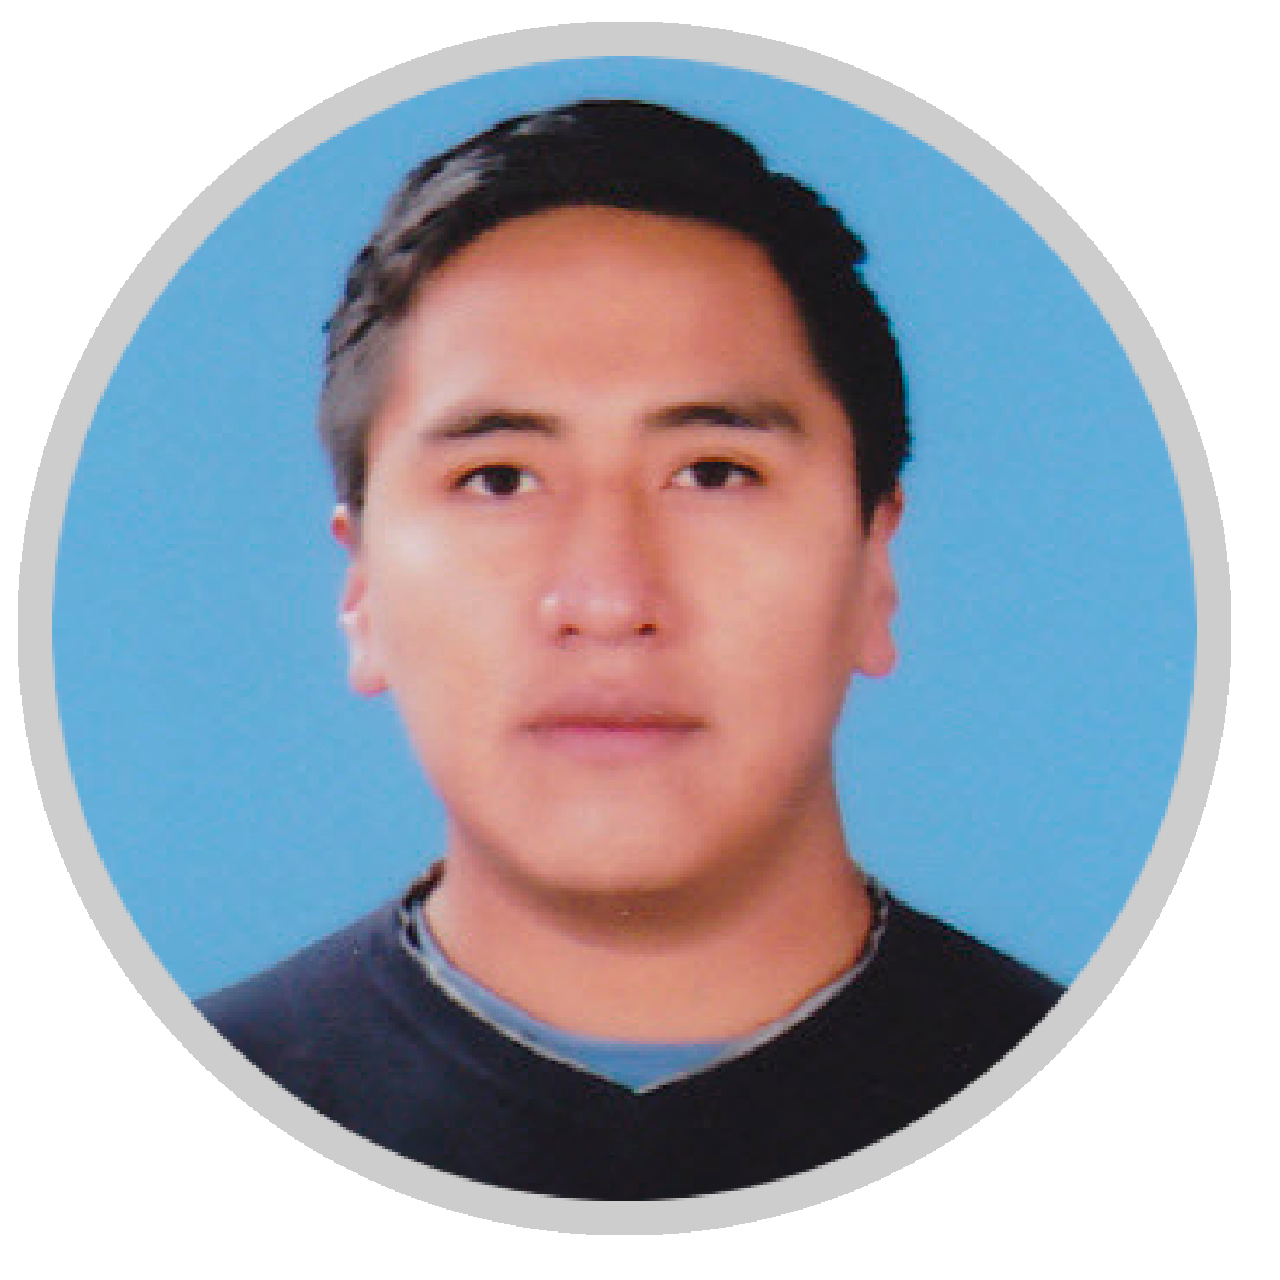
\includegraphics[scale=0.12]{images/Marco-3}\\
			\textbf{Marco Antonio Vino Chipana}\\\\
			\href{https://www.linkedin.com/in/mavino/}{
\includegraphics[scale=0.04]{images/linkedin_logo}} mavino
		}
	}
}
\colorbox{white}{
	\makebox[7.5in][l]{
		\shortstack[c]{
			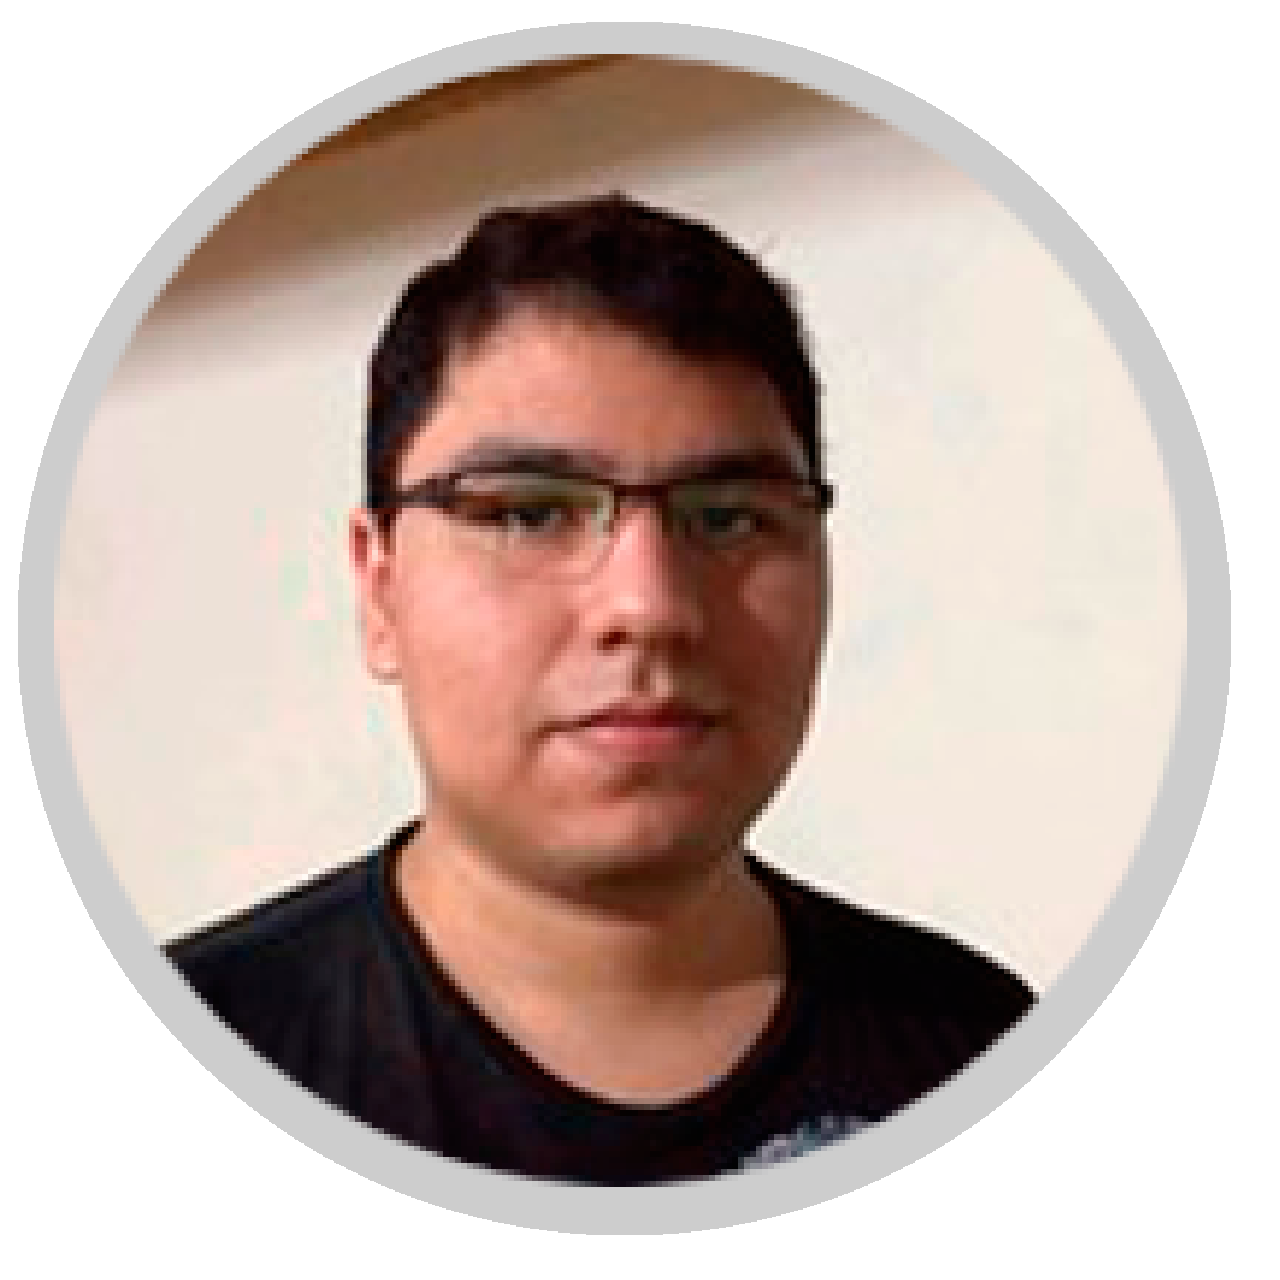
\includegraphics[scale=0.12]{images/rafa-3}\\
			\textbf{Rafael Villca Poggian}\\\\
			\href{https://www.linkedin.com/in/rvillca/}{
\includegraphics[scale=0.04]{images/linkedin_logo}} rvillca
		}
	}
}
\newpage

\newgeometry{margin = 0in}
\hspace*{1.5cm}
\colorbox{white}{%
	\shortstack[r]{
		\makebox[8.5in][r]{\shortstack[r]{\vspace{1 in}}}\\
		\parbox{8.5in}{%
			\section*{\fontsize{25}{25}\rmfamily\color{celeste}4. Contacto y registro}
			\vspace*{1.5cm}
			\fontsize{15}{15}\rmfamily\color{celeste}
			\begin{itemize}%
					\item \textbf{Grupo de Facebook:} %\url{https://goo.gl/3xUW18}\\
					\rurl{bit.ly/LaPazSchoolOfAI}\\
					\hspace*{1.65in}
\includegraphics[scale=0.060]{images/QR_Code_Grupo_La_Paz_School_of_AI}
					\item \textbf{Formulario de Registro:} %\url{https://goo.gl/zHyjiJ}\\
					\rurl{bit.ly/RegistroISML}\\
					\hspace*{1.65in}
\includegraphics[scale=0.060]{images/QR_Code_Formulario}
			\end{itemize}%
		}%
		\\
		\makebox[8.5in][r]{\shortstack[r]{\vspace{0.3 in}}}
	}
}
\vspace{0.82 cm}\\
\begin{center}
{\fontsize{14}{14}\rmfamily\color{black}    Con el apoyo de:}\\
\end{center}
\colorbox{gris1}{\makebox[8.5in][c]{\shortstack[c]{
\parbox{8.5in}{
\begin{center}

\includegraphics[scale=0.08]{images/ESTADISTICA}
\hspace{3.5 cm}

\includegraphics[scale=0.09]{images/CEFAC}
\hspace{4 cm}

\includegraphics[scale=0.28]{images/INFORMATICA}
\end{center}
}
}}}
\end{document}
